\documentclass{article}

\usepackage{amsmath,amssymb}
\usepackage{tikz}
\usetikzlibrary{er,positioning}
\usepackage{pgfplots}
\usepackage{xcolor}
\usepackage[left=2.1cm,right=3.1cm,bottom=3cm,footskip=0.75cm,headsep=0.5cm]{geometry}
\usepackage{enumerate}
\usepackage{enumitem}
\usepackage{marvosym}
\usepackage{tabularx}

\usepackage{listings}
\definecolor{lightlightgray}{rgb}{0.95,0.95,0.95}
\definecolor{lila}{rgb}{0.8,0,0.8}
\definecolor{mygray}{rgb}{0.5,0.5,0.5}
\definecolor{mygreen}{rgb}{0,0.8,0.26}
\lstdefinestyle{java} {language=java}
\lstset{language=java,
	basicstyle=\ttfamily,
	keywordstyle=\color{lila},
	commentstyle=\color{lightgray},
	stringstyle=\color{mygreen}\ttfamily,
	backgroundcolor=\color{white},
	showstringspaces=false,
	numbers=left,
	numbersep=10pt,
	numberstyle=\color{mygray}\ttfamily,
	identifierstyle=\color{blue},
	xleftmargin=.1\textwidth, 
	%xrightmargin=.1\textwidth,
	escapechar=§,
}

\usepackage[utf8]{inputenc}

\renewcommand*{\arraystretch}{1.4}

\newcolumntype{L}[1]{>{\raggedright\arraybackslash}p{#1}}
\newcolumntype{R}[1]{>{\raggedleft\arraybackslash}p{#1}}
\newcolumntype{C}[1]{>{\centering\let\newline\\\arraybackslash\hspace{0pt}}m{#1}}

\newcommand{\E}{\mathbb{E}}
\DeclareMathOperator{\rk}{rk}
\DeclareMathOperator{\Var}{Var}
\DeclareMathOperator{\Cov}{Cov}

\title{\textbf{Datenbanken, Übung 3}}
\author{\textsc{Henry Haustein}}
\date{}

\begin{document}
	\maketitle
	
	\section*{Aufgabe 1}
	\begin{enumerate}[label=(\alph*)]
		\item Die Relationen sind
		\begin{itemize}
			\item User(\underline{id}, name)
			\item Tweet(\underline{id}, date, text, writtenBy)
			\item follows(user.id, user.id)
			\item likes(user.id, tweet.id, date)
		\end{itemize}
		\item Ich wüsste nicht, was man noch reduzieren könnte. Wenn man in (a) die Relationen anders aufgebaut hätte, also z.B. eine writes-Relation, dann könnte man hier mein Ergebnis aus (a) hinschreiben können.
		\item Ja. Nein, da mehrere User einen Tweet an unterschiedlichen Tagen liken können. Welchen Wert soll dann \textit{tweet.date} annehmen?
	\end{enumerate}

	\section*{Aufgabe 2}
	Das ER-Diagramm
	\begin{center}
		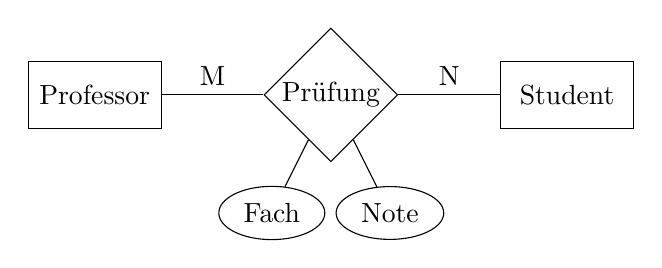
\begin{tikzpicture}
			\node[entity] at (0,0) (p) {Professor};
			\node[entity] at (6,0) (s) {Student};
			\node[relationship] at (3,0) (pr) {Prüfung}
				child{node[attribute] {Fach}}
				child{node[attribute] {Note}};
			
			\draw (p) to node[above] {M} (pr) to node[above] {N} (s);
		\end{tikzpicture}
	\end{center}
	Mehrere Fächer sollten kein Problem darstellen, problematisch sind hier Wiederholungsprüfungen. Bei mehrfachen Eintragungen in die Datenbank wüsste man nicht, was die aktuelle Note des Studenten in einem Fach ist. Hat der Student das Studium abgebrochen (5.0 bleibt stehen) oder gibt es eine bestandene Wiederholungsprüfung (5.0 bleibt nicht bestehen). Man könnte Prüfungen mit Note 5.0 einfach nicht in die Datenbank aufnehmen, könnte dann aber nicht zählen, wie viele Versuche ein Student bereits gebraucht hat. Einfachste Lösung wäre hier wohl ein zusätzliches Attribut \textit{status}, welches speichert, ob die Prüfung angenommen wurde, eine Wiederholungsklausur geschrieben wurde, das Studium abgebrochen wurde, ...


	\section*{Aufgabe 3}
	\begin{enumerate}[label=(\alph*)]
		\item Es gilt $A\to B\times C$, $A\times C\to B$ und $A\times B\to C$.
		\item Die Relationen sind
		\begin{itemize}
			\item A(\underline{a\_id})
			\item B(\underline{b\_id})
			\item C(\underline{c\_id})
			\item R(a\_id, b\_id, c\_id)
		\end{itemize}
		\item Wäre es nicht sinnvoll einfach eine Relation A(a\_id,b\_id,c\_id) zu machen?
		\item ?
	\end{enumerate}
	
	\section*{Aufgabe 4}
	\begin{enumerate}[label=(\alph*)]
		\item Ist das nicht das selbe wie in (b)?
		\item Es gilt:
		\begin{itemize}
			\item Universalrelation: $R(A_1,A_2,A_3)$
			\item vertikale Zerlegung: $R_1(A_1,A_2)$, $R_2(A_3, \text{Bezug zu X})$
			\item horizontale Zerlegung: $R_1(A_1,A_2)$, $R_2(A_1,A_2,A_3)$
		\end{itemize}
	\end{enumerate}
	
\end{document}